\begin{frame}
	\frametitle{Sampling Planning Overview}

	\begin{columns}
		\column{0.5\textwidth}
			RRT-based approach
			\begin{itemize}
				\item
					Sample poses directly

					\begin{equation*}
						\pose = (\transvec, \quaternion)
					\end{equation*}

				\item

					Translation drawn from normal distribution:

					\begin{itemize}

						\item

							Capacity margin higher towards center of workspace

						\item

							Median in center of workspace

						\item

							Edges are three standard deviations away from the
							median

					\end{itemize}
			\end{itemize}
		\column{0.5\textwidth}
			\begin{itemize}

				\item

					Orientation:

					\begin{itemize}

							\item

								Angle from normal distribution:

								median: $\pi/2$

								Standard deviation $\pi/6$

							\item

								Quaternion formula:

								\begin{equation*}
									\quaternion = \sin(\theta/2)\vec{j} +
									\cos(\theta/2)
								\end{equation*}

					\end{itemize}
			\end{itemize}

			\begin{figure}[hb]
				\centering
				\def\svgwidth{\columnwidth}
				\import{res/img/}{pose_sampling.pdf_tex}
				\caption{Pose Sampling}%
				\label{fig:pose_sampling}
			\end{figure}
	\end{columns}
\end{frame}

\begin{frame}
	\frametitle{Capacity Margin}

	Increase capacity margin at sampled poses:

	\begin{equation*}
		\pose \gets \pose +
		\gain\frac{\nabla\capacitymargin}{\norm{\nabla\capacitymargin}}
	\end{equation*}

	\begin{center}
		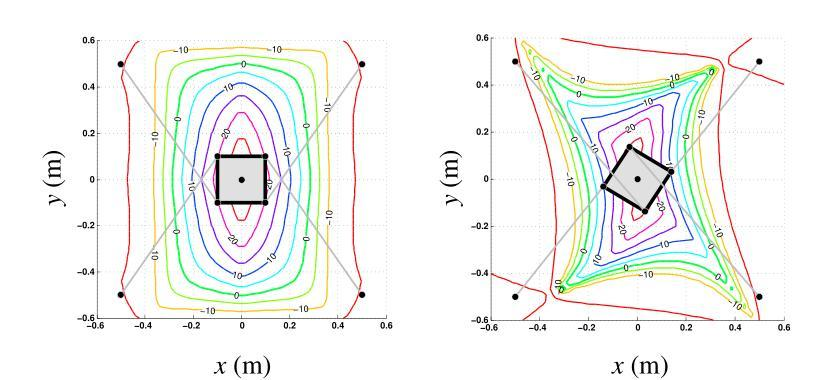
\includegraphics[width=0.8\textwidth]{capacity_margin_isocontours}
		\captionof{figure}{Capacity Margin Isocontours~\cite{bib:cdpr:measuring_how_well_a_structure_supports_varying_external_wrenches}}
	\end{center}
	\end{columns}
\end{frame}

\begin{frame}
	\frametitle{Distance Measure in $\specialEuclideanGroup{3}$}

	Measure distance in cable space:

	\begin{equation*}
		\dist(\pose_1, \pose_2) =
			\norm{%
				\invgeometricmodel(\pose_2) - \invgeometricmodel(\pose_1)
			}
		\label{eq:distance_measure}
	\end{equation*}

	Advantage:

	\begin{itemize}
		\item Dimensionally homogeneous measure of both orientation and
			translational distances.
	\end{itemize}

	Incorporating the capacity margin:

	\begin{equation*}
		\dist(\pose_1, \pose_2) =
			-\gain_{\capacitymargin}
			\frac%
			{%
				\capacitymargin(\pose_2) - \capacitymargin(\pose_1)
			}
			{%
				%\int_{\pathsym} \der\pose
				%\int_0^1 \capacitymargin(\pathsym(\timenorm))\der\timenorm
				\forcemag_{\max}
			}
			+
			(1 - \gain_{\capacitymargin})
			\frac%
			{%
				\norm{%
					\invgeometricmodel(\pose_2) - \invgeometricmodel(\pose_1)
				}
			}
			{%
				\diag(\workspace)
			}
			\label{eq:distance_measure_capcity_margin}
	\end{equation*}
\end{frame}
